Using the learnt \otnn~on FashionMNIST, CelebA (Mouth Slightly Open label), Cat vs Dog and Imagenet, Fig.~\ref{fig:celebA_counterfactual},\ref{fig:fashionMNIST_counterfactual}  present the original image, average gradients $\nabla_x f_j$  over the channels, and images in the direction of the transport plan (Prop.~\ref{th:gradient_transport_plan}), other samples are given in Appendix~A.5. 
We can see that most of the gradients are visually consistent, showing clearly what has to be changed in the input image to modify the class and act as a counterfactual explanation. 
%what needed to change in the input image to classes and act as a counterfactual explanation. 
This is less clear for the Imagenet examples. This could be due to the difficulty of defining a transport plan for each pair of the 1000 classes. However, feature visualizations in Figure \ref{fig:big_picture} show that the internal representation of the classes is still more interpretable than the unconstraint one. 
More generally, we observe that the gradient gives clear information about how the classifier makes its decision. For instance, for the cat, it shows that the classifier does not need to encode perfectly the concept of a cat, but mainly to identify the color of the eyes and size of the nose.
%\commentgreen{@Mathieu tu en feras d'autres images sinon enlever la paranthese}

\iffalse
\begin{figure*}
    \centering
        \begin{tabular}{ccc}
        \multicolumn{3}{c}{CelebA Mouth Slightly Open label: left close to open, right open to close} \\
        \begin{tabular}{ccc}
            \includegraphics[width=.13\linewidth]{img/Mouth_slightly_open/00024_input_lbl0_fx-0.59.pdf} & \includegraphics[width=.13\linewidth]{img/Mouth_slightly_open/00024_gradColor.pdf} & \includegraphics[width=.13\linewidth]{img/Mouth_slightly_open/00024_xMinus10.0Grad.pdf} 
        \end{tabular} &
        \begin{tabular}{ccc}
            \includegraphics[width=.13\linewidth]{img/Mouth_slightly_open/00072_input_lbl1_fx0.47.pdf} & \includegraphics[width=.13\linewidth]{img/Mouth_slightly_open/00072_gradColor.pdf} & \includegraphics[width=.13\linewidth]{img/Mouth_slightly_open/00072_xMinus10.0Grad.pdf} 
        \end{tabular} & \\
         %\midrule
          
        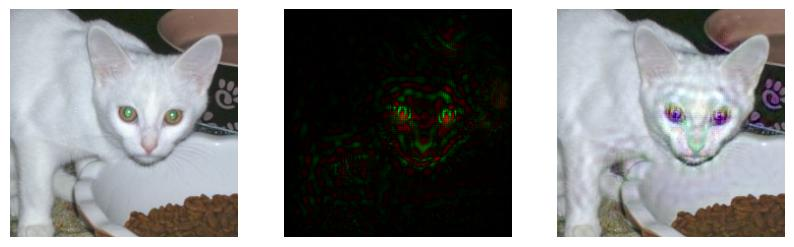
\includegraphics[width=.5\linewidth] {img/catvsdog/expl_1.jpg} &
        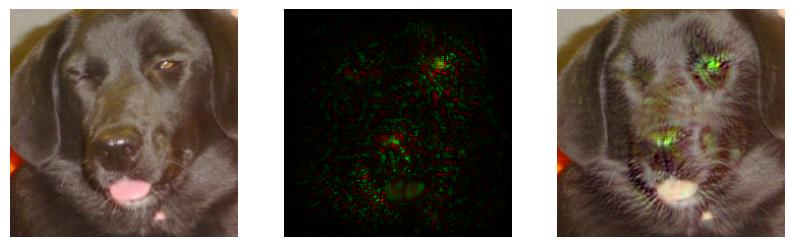
\includegraphics[width=.5\linewidth] {img/catvsdog/expl_2.jpg} & \\
        % \midrule
        \multicolumn{3}{c}{Imagenet :left cabbage butterfly to monarch one,  right great grey owl to bald eagle} \\
        
\includegraphics[width=.5\linewidth] {img/imagenet/expl_1.jpg} &
        
\includegraphics[width=.5\linewidth] {img/imagenet/expl_2.jpg} %\\
        & \\
     \end{tabular}
    \caption{Samples of conterfactuals from different dataset: (left) source image , (center) gradient image, (right) counterfactual of the form $\x-t*\hat{f}(\x)\nabla_x \hat{f}(\x)$, for  $t>1$}
    \label{fig:celebA_counterfactual}
\end{figure*}


\begin{figure*}[h]
  \centering
  \fbox{\includegraphics[width=0.98\linewidth]{img/fashion-otnn.png}}
  
\caption{Samples from different classes of FashionMNIST: (left) source image , (center) targeted gradient image of an \otnn, (right) targeted counterfactual of the form $\x-10*\hat{f}(\x)\nabla_x \hat{f}(\x)$}
%Counterfactuals of the form $ \x-10*\hat{f}(\x)\nabla_x \hat{f}(\x)$  of a \otnn~ for FashionMNIST. }
\label{fig:fashion_mnist}
\end{figure*}
\fi


\begin{figure*}
\centering
\begin{tabular}{ccc}
%\multicolumn{3}{c}{Fashion MNIST source image and class, targeted gradient image and counterfactual.} \\
\multicolumn{3}{c}{\includegraphics[width=1.0\linewidth]{img/fashion-otnn.pdf}}\\
\end{tabular}
\caption{Samples of counterfactuals for FashionMNIST dataset on different classes and targets: (left) source image , (center) gradient image, (right) counterfactual of the form $\x-t*\hat{f}(\x)\nabla_x \hat{f}(\x)$, for  $t>1$}
\label{fig:fashionMNIST_counterfactual}
\end{figure*}

\iftrue
\begin{figure*}
    \centering
    \begin{tabular}{rcc}
        %\multicolumn{3}{c}{Fashion MNIST source image and class, targeted gradient image and counterfactual.} \\
        %\multicolumn{3}{c}{\includegraphics[width=1.0\linewidth]{img/fashion-otnn.pdf}}\\
        %\multicolumn{3}{c}{CelebA Mouth Slightly Open label: left close to open, right open to close} \\
        \rotatebox[origin=c]{90}{CelebA}\hspace{-5mm} & 
        \begin{tabular}{ccc}
            \includegraphics[width=.13\linewidth]{img/Mouth_slightly_open/00024_input_lbl0_fx-0.59.pdf} & \includegraphics[width=.13\linewidth]{img/Mouth_slightly_open/00024_gradColor.pdf} & \includegraphics[width=.13\linewidth]{img/Mouth_slightly_open/00024_xMinus10.0Grad.pdf}\\
            % \textbf{mouth closed} & $\to$ & \textbf{mouth opened}
        \end{tabular} &
        \begin{tabular}{ccc}
            \hspace{-4mm}
            \includegraphics[width=.13\linewidth]{img/Mouth_slightly_open/00072_input_lbl1_fx0.47.pdf} & \includegraphics[width=.13\linewidth]{img/Mouth_slightly_open/00072_gradColor.pdf} & \includegraphics[width=.13\linewidth]{img/Mouth_slightly_open/00072_xMinus10.0Grad.pdf} \\
            % \textbf{mouth opened} & $\to$ & \textbf{mouth closed}
        \end{tabular} \\
          & \textbf{mouth closed $\to$ mouth opened} &  \textbf{mouth opened $\to$ mouth closed}\\
        %\midrule
        % \multicolumn{3}{c}{CelebA Blurry label: left blurry to not blurry, right not blurry to blurry} \\
        %%%%%%%%%%%%%%%%%%%%%%%%%
        \rotatebox[origin=c]{90}{CelebA}\hspace{-5mm} & 
        \begin{tabular}{ccc}
            \includegraphics[width=.13\linewidth]{img/samplesAppendix/Blurry/00027_input_lbl1_fx0.72.pdf} & \includegraphics[width=.13\linewidth]{img/samplesAppendix/Blurry/00027_gradColor.pdf} & \includegraphics[width=.13\linewidth]{img/samplesAppendix/Blurry/00027_xMinus10.0Grad.pdf}\\
            % \textbf{blurry} & $\to$ & \textbf{not blurry}
        \end{tabular} &
        \begin{tabular}{ccc}
            \hspace{-4mm}
            \includegraphics[width=.13\linewidth]{img/samplesAppendix/Blurry/00250_input_lbl0_fx-1.15.pdf} & \includegraphics[width=.13\linewidth]{img/samplesAppendix/Blurry/00250_gradColor.pdf} & \includegraphics[width=.13\linewidth]{img/samplesAppendix/Blurry/00250_xMinus5.0Grad.pdf}\\
            % \textbf{not blurry} & $\to$ & \textbf{blurry}
        \end{tabular} \\
          & \textbf{blurry $\to$ not blurry} & \textbf{not blurry $\to$ blurry}\\
        %\midrule
        % \multicolumn{3}{c}{CelebA Rosy cheeks label: rosy to not rosy, right not rosy to rosy} \\
        %%%%%%%%%%%%%%%%%%%%%%%%%%%%%%%%%%%%%
        \rotatebox[origin=c]{90}{CelebA}\hspace{-5mm} & 
        \begin{tabular}{ccc}
            \includegraphics[width=.13\linewidth]{img/samplesAppendix/Rosy_Cheeks/00132_input_lbl1_fx3.26.pdf} & \includegraphics[width=.13\linewidth]{img/samplesAppendix/Rosy_Cheeks/00132_gradColor.pdf} & \includegraphics[width=.13\linewidth]{img/samplesAppendix/Rosy_Cheeks/00132_xMinus2.5Grad.pdf}\\
            % \textbf{rosy cheeks} & $\to$ & \textbf{w/o rosy cheeks}
        \end{tabular} &
        \begin{tabular}{ccc}
            \hspace{-4mm}
            \includegraphics[width=.13\linewidth]{img/samplesAppendix/Rosy_Cheeks/00079_input_lbl0_fx-7.52.pdf} & \includegraphics[width=.13\linewidth]{img/samplesAppendix/Rosy_Cheeks/00079_gradColor.pdf} & \includegraphics[width=.13\linewidth]{img/samplesAppendix/Rosy_Cheeks/00079_xMinus2.0Grad.pdf}\\
            % \textbf{w/o rosy cheeks} & $\to$ & \textbf{rosy cheeks}
        \end{tabular} \\
        & \textbf{rosy cheeks $\to$ w/o rosy cheeks} & \textbf{w/o rosy cheeks $\to$ rosy cheeks}\\
        %\midrule 
        %\multicolumn{3}{c}{Cat vs dog : left cat to dog, right dog to cat} \\
        \rotatebox{90}{\quad Cat vs Dog}\hspace{-5mm} &
        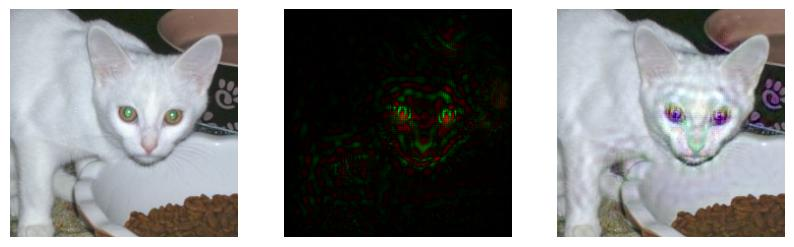
\includegraphics[width=.464\linewidth] {img/catvsdog/expl_1.jpg} &
            \hspace{-4mm}
        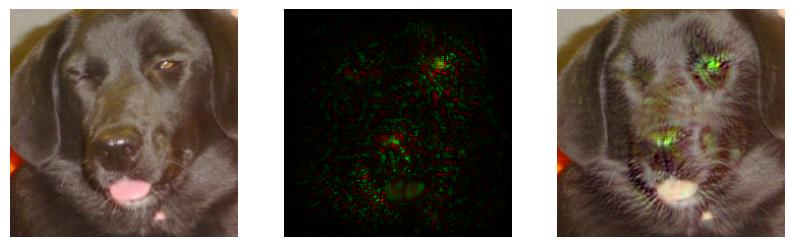
\includegraphics[width=.464\linewidth] {img/catvsdog/expl_2.jpg}\\
        & \textbf{cat $\to$ dog} & \textbf{dog $\to$ cat}\\
        % \midrule
        % \multicolumn{3}{c}{Imagenet :left cabbage butterfly to monarch one,  right great grey owl to bald eagle} \\
        \rotatebox{90}{\quad Imagenet}\hspace{-5mm} &
        
\includegraphics[width=.464\linewidth] {img/imagenet/expl_1.jpg} &
            \hspace{-4mm}
        
\includegraphics[width=.464\linewidth] {img/imagenet/expl_2.jpg} \\
        & \textbf{cabbage butterfly $\to$ monarch butterfly} & \textbf{great grey owl $\to$ bald eagle}\\
     \end{tabular}
    \caption{Samples of counterfactuals from different datasets: (left) source image , (center) gradient image, (right) counterfactual of the form $\x-t*\hat{f}(\x)\nabla_x \hat{f}(\x)$, for  $t>1$}
    \label{fig:celebA_counterfactual}
\end{figure*}
\fi

